\documentclass[a4paper]{article}

\usepackage{INTERSPEECH_v2}
\usepackage{lipsum} % we can remove this at the end

\title{Paper Template for INTERSPEECH}
\name{Author Name$^1$, Co-author Name$^2$}
\address{
  $^1$Author Affiliation, Sweden\\
  $^2$Co-author Affiliation, Australia}
\email{author@university.edu, coauthor@company.com}

\begin{document}

\maketitle
% 
\begin{abstract}
% Copyright (C) 2016  Arvid Fahlström Myrman
%
% This program is free software; you can redistribute it and/or modify
% it under the terms of the GNU General Public License as published by
% the Free Software Foundation; either version 2 of the License, or
% (at your option) any later version.
%
% This program is distributed in the hope that it will be useful,
% but WITHOUT ANY WARRANTY; without even the implied warranty of
% MERCHANTABILITY or FITNESS FOR A PARTICULAR PURPOSE.  See the
% GNU General Public License for more details.
%
% You should have received a copy of the GNU General Public License along
% with this program; if not, write to the Free Software Foundation, Inc.,
% 51 Franklin Street, Fifth Floor, Boston, MA 02110-1301 USA.

\begin{abstract}
  English abstract goes here.
  \lipsum[1-2]
\end{abstract}

\clearpage

\begin{otherlanguage}{swedish}
  \begin{abstract}
    Träutensilierna i ett tryckeri äro ingalunda en faktor där
    trevnadens ordningens och ekonomiens upprätthållande, och dock är
    det icke sällan som sorgliga erfarenheter göras ordningens och
    ekon och miens därmed upprätthållande. Träutensilierna i ett
    tryckeri äro ingalunda en oviktig faktor, för trevnadens
    ordningens och och dock är det icke sällan.
  \end{abstract}
\end{otherlanguage}

\cleardoublepage

\end{abstract}
% check these
\noindent\textbf{Index Terms}: zero-resource speech challenge, unsupervised learning, speech recognition

% Copyright (C) 2016  Arvid Fahlström Myrman
%
% This program is free software; you can redistribute it and/or modify
% it under the terms of the GNU General Public License as published by
% the Free Software Foundation; either version 2 of the License, or
% (at your option) any later version.
%
% This program is distributed in the hope that it will be useful,
% but WITHOUT ANY WARRANTY; without even the implied warranty of
% MERCHANTABILITY or FITNESS FOR A PARTICULAR PURPOSE.  See the
% GNU General Public License for more details.
%
% You should have received a copy of the GNU General Public License along
% with this program; if not, write to the Free Software Foundation, Inc.,
% 51 Franklin Street, Fifth Floor, Boston, MA 02110-1301 USA.

% \begin{figure}
%   \centering
%   Sound + transcription + posteriorgrams
% 
%   \caption{\label{fig:postspec}Posteriorgram spectrum}
% \end{figure}

\chapter{Introduction}
\section{Background}
Automatic speech recognition (ASR) is generally framed as a supervised task, where both acoustic speech data and the corresponding transcription is available, and the problem is to develop a model that can mimic this mapping from speech to text.
However, developing such data is expensive, both in terms of time and money, as it involves painstakingly transcribing many hours of speech.
As a result, there is a notable lack of high-quality data for speech recognition for a majority of languages around the world.
An important question is thus whether it is possible to make use of untranscribed, or unlabelled, data to develop ASR for such low-resource languages.
Unsupervised learning in this manner may also provide insight into the linguistic structure of languages, or the language acquisition of infants.

We focus in particular on one aspect of unsupervised learning of speech, namely the discovery of phonetic classes, i.e.\ the basic speech sounds that make up all words in a language.
While supervised speech recognition makes use of prior knowledge regarding what sounds are present in a language, in unsupervised acquisition of speech this knowledge is unavailable to us.
This means that not only do we need to be able to discover what sounds make up each word in a recording without the use of a transcription---we need to discover what sounds are even available in the language to begin with, as not all languages use the same sounds, nor are the same sounds contrastive in all languages.
This is compounded by speaker variation, where there can be significant differences between the pronunciation of sounds by individual speakers, or even by the same speaker depending on e.g.\ the context of the sound.
This variation makes approaches such as naive clustering ineffective, as many of the discovered sounds are likely to be highly speaker-specific.

Unsupervised speech acquisition is an area of active research.
One source of such research is the Zero Resource Speech Challenge \parencite{versteegh2015zero}, which was developed with the goal of finding linguistic units (track 1) or longer recurring word-like fragments (track 2) in speech.
Models are to be trained using only speech data, voice activity information, and speaker identity information.
The main goal of the first track of the challenge is to find robust representations of speech frames where sounds belonging to the same phonetic category are more similar than sounds belonging to different categories; this is also the approach we will take in this work.

% Copyright (C) 2016  Arvid Fahlström Myrman
%
% This program is free software; you can redistribute it and/or modify
% it under the terms of the GNU General Public License as published by
% the Free Software Foundation; either version 2 of the License, or
% (at your option) any later version.
%
% This program is distributed in the hope that it will be useful,
% but WITHOUT ANY WARRANTY; without even the implied warranty of
% MERCHANTABILITY or FITNESS FOR A PARTICULAR PURPOSE.  See the
% GNU General Public License for more details.
%
% You should have received a copy of the GNU General Public License along
% with this program; if not, write to the Free Software Foundation, Inc.,
% 51 Franklin Street, Fifth Floor, Boston, MA 02110-1301 USA.

\chapter{Related work}
\label{ch:related-work}

This \namecref{ch:related-work} provides a brief overview of recent research into unsupervised acoustic modelling.
The approaches discussed here can broadly be divided into two categories: bottom-up approaches that infer the acoustic model directly from the speech frames, and top-down approaches that first segment the speech into syllable- or word-like units, and afterwards try break these units into smaller subword units.

\section{Bottom-up approaches}

As an individual speech frame only make up a fraction of a complete speech sound, it is natural to model and segment the speech using a model that can capture time dependencies, such as a hidden Markov model (HMM), rather than attempt to cluster the speech frames directly.
One issue with this approach, however, is that the number of possible states (i.e.\ subword units) is unknown a priori.

\textcite{varadarajan2008unsupervised} tackle this problem by first defining a one-state HMM, and then iteratively splitting and merging states as needed to account for the data according to a heuristic.
Training stops once the size of the HMM reaches a threshold.
After training, each state in the HMM can be thought to correspond to some allophone (context-dependent variant realisation) of a phoneme.
It should be noted, however, that in order to interpret a given state sequence as a single phoneme, \citeauthor{varadarajan2008unsupervised} train a separate model using labelled speech to perform this mapping.
The method is thus not fully unsupervised.

\textcite{lee2012nonparametric} take a fully probabilistic approach, defining a model that jointly performs segmentation and acoustic modelling.
An infinite mixture model of tri-state HMM-GMMs modelling subword units is defined using the Dirichlet process, and latent variables representing segment boundaries are introduced.
The data can be thought to be generated by repeatedly sampling an HMM to model a segment, sampling a path through the HMM, and for each state in the path sampling a feature vector from the corresponding GMM.
The probability of transitioning from one unit to another is thus not modelled.
Inference of the model is done using Gibbs sampling.

\textcite{siu2014unsupervised} use an HMM of a more classic form to model the data.
An initial transcription of the data in terms of state labels is first generated in an unsupervised manner using a segmental GMM (SGMM).
The HMM and transcription are then iteratively updated, maximising the probability of the model parameters given the transcription, and the transcription given the model parameters.
Note that the number of allowed states are here defined in advance.
$n$-gram statistics are then collected from the transcription and used for tasks such as unsupervised keyword discovery.

Diverging from previous approaches using temporal models, \textcite{chen2015parallel} perform standard clustering of speech frames using an infinite Gaussian mixture model.
After training, the speech frames are represented as posteriorgrams, which have been shown to be more speaker-invariant than other features such as MFCCs \parencite{zhang2010towards}.
Despite the simple approach, this turned out to be the overall best-performing model in the first track of the 2015 Zero Resource Speech Challenge \parencite{versteegh2016zero}.
\textcite{heck2016unsupervised} later further improved on the model by performing clustering in two stages, with an intermediate supervised dimensionality reduction step using the clusters derived from the first clustering step as target classes.

\textcite{synnaeve2016temporal} use a siamese network to create an embedding where speech frames close to each other are considered to belong to the same subword unit, while distant speech frames are said to differ.
A siamese network is a feedforward neural network that takes two inputs and adjusts its parameters to either maximise or minimise the similarity of the corresponding outputs \parencite{bromley1994signature}.

\section{Top-down approaches}
\todo[inline]{remove information already included in the introduction}

Top-down approaches start by first finding pairs of longer word-like segments using unsupervised term discovery (UTD).
This information provides constraints that can be use to find speech frame representations that are more stable within a given subword unit.
The rationale is that while at the frame level the same speech sound can seem quite different between different speakers or even different realisations of the sound by the same speaker, patterns over a longer duration of time are easier to identify; this idea is illustrated in \textcite{jansen2013weak}.

The UTD systems used in this context are generally based on the segmental dynamic time warping (S-DTW) developed by \textcite{park2008unsupervised}.
S-DTW works by repeatedly performing DTW on two audio streams while constraining the maximum amount of warping allowed, each time changing the starting point of the DTW in both streams.
This yields a set of alignments, from which the stretches of lowest average dissimilarity in each alignment can be extracted.
Unfortunately, this approach is inherently $O(n^2)$ in time.
To remedy this, \textcite{jansen2011efficient} introduced an approximate version that uses binary approximations of the feature vectors to perform the calculations in $O(n \log n)$ time using sparse similarity matrices; this system also serves as the baseline for the second track of the Zero Resource Speech Challenge \parencite{versteegh2015zero}.

\textcite{jansen2011towards} describe a method for finding subword units, assuming that clusters corresponding to words, each cluster containing multiple examples of that word in the form of audio, are given.
For each word, an HMM is trained on all the corresponding examples, the number of states in the model being set to a number proportional to the average duration of the word.
The states from each HMM are then collected and clustered based on the similarity of their distributions, forming clusters that hopefully correspond to subword units.

\textcite{jansen2013weak} take somewhat of an inverse approach, starting by clustering the whole data on a frame level, with the assumption that each cluster will tend to correspond to some speaker- or context-dependent subword unit.
They then look at pairs of word-like segments known to be of the same type and calculate how often clusters tend to co-occurr.
The clusters are then partitioned so that clusters that co-occurr often are placed in the same partition.

\textcite{synnaeve2014phonetics} introduce a neural network known referred to as the ABnet, based on siamese networks \parencite{bromley1994signature}.
The network takes a pair of speech frames as input, and adjusts its parameters so that the outputs are collinear if the inputs are known to correspond to the same subword unit, and orthogonal otherwise, using a cosine-based loss function.
\textcite{thiolliere2015hybrid} made use of this approach in the Zero Resource Speech Challenge, also incorporating unsupervised term discovery so as to make the whole process unsupervised, yielding competitive results \parencite{versteegh2016zero}.
\textcite{zeghidour2016deep} experiment with supplying the ABnet with scattering spectrum features instead of filter bank features, showing that with the right features, a shallow architecture may outperform a deep architecture, especially when the amount of available data is low.

\textcite{kamper2015unsupervised} use an autoencoder-like structure, where a neural network is trained to ``reconstruct'' a frame given another frame known to be of the same type.
\textcite{renshaw2015comparison} used this architecture in the Zero Resource Speech Challenge, albeit with a deeper decoder.

\section{This thesis}
\todo[inline]{make description more application agnostic?}

Two of the most successful approaches so far are the clustering approach of \textcite{chen2015parallel} and the siamese network approach of \textcite{thiolliere2015hybrid}.
We pose the question of whether it is possible to combine the two approaches by first clustering the data in an unsupervised manner using a probabilistic model, and then improving the resulting posteriorgrams using speech fragment information.
This way we are able to take advantage of both the whole unlabelled data set, and the smaller set of discovered fragments.

Many probabilistic models, such as Gaussian mixture models and hidden Markov models, have a concept of latent states or classes.
We pose the problem of improving posteriorgrams from such a model as one of merging, or partitioning, these classes.
By first training the model in a fully unsupervised manner, it learns classes that can generally be assumed to be highly speaker-specific.
We can then use weak supervision to merge these classes, yielding representations that are more speaker invariant.

A partitioning of classes can be viewed as a surjection from the original set of classes to a class set of lower cardinality, but finding this surjection is a discrete problem which is difficult to optimise for.
However, a benefit of posteriorgrams is that the probability of an output class can be described as a simple sum of the probabilities of the classes that map to the class in question.
This means that the surjection can be approximated using a continuous linear model which can be optimised through standard gradient descent.
A linear model also has the added benefit of being more interpretable than deep networks such as that of \textcite{thiolliere2015hybrid}.
While the approach of partitioning posteriorgrams is very reminiscent of \textcite{jansen2013weak}, the major difference is that in place of direct clustering of classes, we are instead trying to maximise the similarity/dissimilarity between pairs of speech fragments, which only indirectly results in a partitioning of the classes.


\section{This thesis}

\begin{figure}
  \centering
  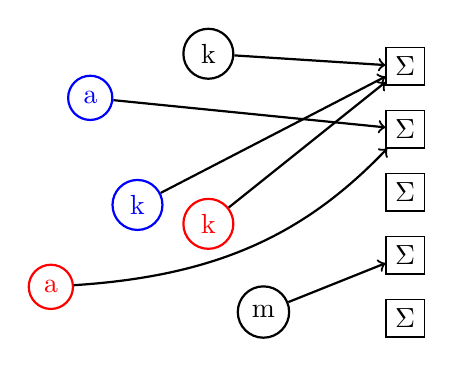
\begin{tikzpicture}[outpos/.style={draw,rectangle},inpos/.style={draw,circle,thick},
    arr/.style={->,thick},yscale=0.8]
    \node[outpos] at (0,0) {$\Sigma$};
    \node[outpos] (out3) at (0,1) {$\Sigma$};
    \node[outpos] at (0,2) {$\Sigma$};
    \node[outpos] (out2) at (0,3) {$\Sigma$};
    \node[outpos] (out1) at (0,4) {$\Sigma$};
    
    \node[inpos,blue] (a1) at (-4, 3.5) {a};
    \node[inpos,red] (a2) at (-4.5, 0.5) {a};
    \node[inpos,blue] (k1) at (-3.4, 1.8) {k};
    \node[inpos,red] (k2) at (-2.5, 1.5) {k};
    \node[inpos] (k3) at (-2.5, 4.2) {k};
    \node[inpos] (m1) at (-1.8, 0.1) {m};
    
    \draw (a1) edge[arr] (out2) (a2) edge[arr,bend right=24] (out2)
          (k1) edge[arr] (out1) (k2) edge[arr] (out1) (k3) edge[arr] (out1)
	  (m1) edge[arr] (out3);
  \end{tikzpicture}

  \caption{\label{fig:mapping}An example of merging speaker-specific (coloured) clusters by mapping them to (a subset of) the available outputs.
  As we represent the input as a probability vector, each output is a simple sum of the input probabilities.}
\end{figure}

We take inspiration from two of the most successful approaches so far: the clustering approach of \textcite{chen2015parallel} and the siamese network approach of \textcite{thiolliere2015hybrid}, described above.
We pose the question of whether it is possible to combine the two approaches.
One way to do this is to first cluster the whole data set in a fully unsupervised manner, discovering latent classes from the data such that similar data points belong to the same latent class.
By extracting a latent representation of the data from the clustering model, we can then improve on this representation using speech fragment information.
This way we are able to take advantage of both the complete unlabelled data set, and the smaller set of discovered fragments.

For this work we consider in particular probabilistic models such as Gaussian mixture models and hidden Markov models.
These models express class membership in terms of probabilities, giving the posterior probability of each data point belonging to one of the latent classes.
By representing each data point as a vector of these posterior probabilities, called a posteriorgram, the task of improving this representation can be framed as one of merging, or partitioning, the latent classes appropriately.
Latent classes discovered through unsupervised training will generally be highly speaker-specific.
However, by merging the classes using weak supervision in the form of speech fragment pairs, we can construct classes that are more speaker invariant.

A partitioning of classes can be viewed as finding a function which maps the original set of classes to a class set of lower cardinality, but finding this function is a discrete problem which is difficult to optimise for.
However, a benefit of posteriorgrams is that the probability of an output class can be described as a simple sum of the probabilities of the input classes that map to the output in question, as illustrated in \cref{fig:mapping}.
This means that the mapping function can be approximated using a continuous linear model which can be optimised through standard gradient descent.
A linear model also has the added benefit of being more interpretable than deep networks such as that of \textcite{thiolliere2015hybrid}.
While the approach of partitioning posteriorgrams is very reminiscent of \textcite{jansen2013weak}, the major difference is that in place of direct clustering of classes, we are instead trying to maximise the similarity/dissimilarity between pairs of speech fragments, which only indirectly results in a partitioning of the classes.

\begin{figure}
  \centering
  \begin{tikzpicture}
    %\begin{axis}[enlargelimits=false,axis on top,width=8cm,height=4cm,ylabel={Frequency (\si\Hz)},xlabel={Time (\si\s)}]
    %\end{axis}

% speaker 1
% s3102b 146.518752 147.111647 questions
%   146.518752  122 ng
%   146.596735  122 k
%   146.624258  122 w
%   146.693066  122 ah
%   146.760727  122 s; *
%   146.816920  122 ch
%   147.021050  122 en
%   147.111647  122 z

% speaker 2
% s2302a 106.778375 107.628939 questions
%   106.778375  122 ng
%   106.883302  122 k
%   106.921215  122 w
%   106.985553  122 eh
%   107.098375  122 s ; *
%   107.168375  122 ch
%   107.246360  122 ah
%   107.348375  122 n
%   107.628939  122 z
    \begin{groupplot}[group style={group size=2 by 3, horizontal sep=2cm, vertical sep=0.4cm},
      enlargelimits=false,width=6.5cm,height=5.7cm,axis on top,xtick=\empty]
      \nextgroupplot[ylabel={Frequency (\si\Hz)},title={Female speaker}]
      \addplot graphics[xmin=146.52,xmax=147.11,ymin=0,ymax=3125] {data/spectrum-speaker-1-crop.pdf};
      \coordinate (kw1t) at (axis cs:146.59,\pgfkeysvalueof{/pgfplots/ymax});
      \coordinate (we1t) at (axis cs:146.62,\pgfkeysvalueof{/pgfplots/ymax});
      \coordinate (es1t) at (axis cs:146.69,\pgfkeysvalueof{/pgfplots/ymax});
      \coordinate (sc1t) at (axis cs:146.76,\pgfkeysvalueof{/pgfplots/ymax});
      \coordinate (cu1t) at (axis cs:146.82,\pgfkeysvalueof{/pgfplots/ymax});
      \coordinate (un1t) at (axis cs:147.02,\pgfkeysvalueof{/pgfplots/ymax});

      \nextgroupplot[title={Male speaker}]
      \addplot graphics[xmin=106.78,xmax=107.63,ymin=0,ymax=3125] {data/spectrum-speaker-2-crop.pdf};
      \coordinate (kw2t) at (axis cs:106.88,\pgfkeysvalueof{/pgfplots/ymax});
      \coordinate (we2t) at (axis cs:106.92,\pgfkeysvalueof{/pgfplots/ymax});
      \coordinate (es2t) at (axis cs:106.99,\pgfkeysvalueof{/pgfplots/ymax});
      \coordinate (sc2t) at (axis cs:107.10,\pgfkeysvalueof{/pgfplots/ymax});
      \coordinate (cu2t) at (axis cs:107.17,\pgfkeysvalueof{/pgfplots/ymax});
      \coordinate (un2t) at (axis cs:107.35,\pgfkeysvalueof{/pgfplots/ymax});
      
      \nextgroupplot[ylabel={GMM component}]
      \addplot graphics[xmin=146.52,xmax=147.11,ymin=1,ymax=1024] {data/gmm-posteriorgrams-speaker-1-crop.pdf};
      
      \nextgroupplot
      \addplot graphics[xmin=106.78,xmax=107.63,ymin=1,ymax=1024] {data/gmm-posteriorgrams-speaker-2-crop.pdf};
      
      \nextgroupplot[ylabel={Model output},xlabel={Time}]
      \addplot graphics[xmin=146.52,xmax=147.11,ymin=1,ymax=33] {data/reduced-posteriorgrams-speaker-1-crop.pdf};
      \coordinate (kw1b) at (axis cs:146.59,\pgfkeysvalueof{/pgfplots/ymin});
      \coordinate (we1b) at (axis cs:146.62,\pgfkeysvalueof{/pgfplots/ymin});
      \coordinate (es1b) at (axis cs:146.69,\pgfkeysvalueof{/pgfplots/ymin});
      \coordinate (sc1b) at (axis cs:146.76,\pgfkeysvalueof{/pgfplots/ymin});
      \coordinate (cu1b) at (axis cs:146.82,\pgfkeysvalueof{/pgfplots/ymin});
      \coordinate (un1b) at (axis cs:147.02,\pgfkeysvalueof{/pgfplots/ymin});
      
      \nextgroupplot[xlabel={Time}]
      \addplot graphics[xmin=106.78,xmax=107.63,ymin=1,ymax=33] {data/reduced-posteriorgrams-speaker-2-crop.pdf};
      \coordinate (kw2b) at (axis cs:106.88,\pgfkeysvalueof{/pgfplots/ymin});
      \coordinate (we2b) at (axis cs:106.92,\pgfkeysvalueof{/pgfplots/ymin});
      \coordinate (es2b) at (axis cs:106.99,\pgfkeysvalueof{/pgfplots/ymin});
      \coordinate (sc2b) at (axis cs:107.10,\pgfkeysvalueof{/pgfplots/ymin});
      \coordinate (cu2b) at (axis cs:107.17,\pgfkeysvalueof{/pgfplots/ymin});
      \coordinate (un2b) at (axis cs:107.35,\pgfkeysvalueof{/pgfplots/ymin});

  \end{groupplot}
  \draw [thin,white] (kw1t) -- (kw1b);
  \draw [thin,white] (we1t) -- (we1b);
  \draw [thin,white] (es1t) -- (es1b);
  \draw [thin,white] (sc1t) -- (sc1b);
  \draw [thin,white] (cu1t) -- (cu1b);
  \draw [thin,white] (un1t) -- (un1b);
  
  \draw [thin,white] (kw2t) -- (kw2b);
  \draw [thin,white] (we2t) -- (we2b);
  \draw [thin,white] (es2t) -- (es2b);
  \draw [thin,white] (sc2t) -- (sc2b);
  \draw [thin,white] (cu2t) -- (cu2b);
  \draw [thin,white] (un2t) -- (un2b);
  \end{tikzpicture}

  \caption{\label{fig:model-output}Example of using the proposed model to process utterances of the word ``question'' from two different speakers.
  First the energy spectrum is calculated for each speech frame (top).
  After preprocessing the spectrum is then fed to a Gaussian mixture model from which posterior probabilities for each latent class is extracted (middle).
  Last, the probability vectors from the GMM are reduced in size using the proposed model (bottom).
  The white crosses mark the most probable class state for each frame.
  The white vertical lines mark boundaries between speech sounds.
  The example is meant to be illustrative and does not represent the overall performance of the model.}
\end{figure}

Using such a linear model, we hope to use speech fragment information to improve on posteriorgrams obtained from an unsupervised probabilistic model.
In particular we hope to use the model to construct more speaker-invariant posteriorgrams which can be used to discriminate between different linguistic units in a robust manner.
An example of using the model can be seen in \cref{fig:model-output}; the model takes high-dimensional posteriorgrams describing a probability distribution over latent variables (classes) from a Gaussian mixture model, and outputs low-dimensional posteriorgrams which are more speaker invariant.
We evaluate the model using the minimal-pair ABX task used for evaluation in the first track of the Zero Resource Speech Challenge.
The minimal-pair ABX task aims to evaluate the quality of different representations of speech by ensuring that two utterances of the same word are more similar to each other than to a distinct but similar word.

\section{Method}
\label{sec:method}
% Arvid: check that I am not getting this wrong

\todo[inline]{intuitive explanation of what we want to do}
%The goal of our method is to merge acoustic clusters obtained by bottom-up unsupervised classification such that the resulting classes correspond more closely to phonemic units in the language.

%Given two input vectors $\mat x$ and $\mat y$, we wish to determine whether the vectors belong to the same category, or class.
%To do so, we project the vectors onto a space designed so that vectors belonging to the same class are close, while vectors belonging to different classes are distant.
%We consider in particular posteriorgrams---probability vectors $\mat p = (p_1, \dots, p_M)$ representing a posterior distribution over $M$ discrete values.
%The probabilities in $\mat p$ sum to $1$, with $p_i$ being the probability of the $i$th value; for instance, it could be the probability that a data point belongs to the $i$th latent class as inferred by a Gaussian mixture model.

%We assume that the $M$ input probabilities correspond to ``pseudo''-classes (e.g.\ allophones), where several pseudo-classes together describe a single ``true class'' (e.g.\ phonemes).
%Our goal is then to find a function $f$ that maps the $M$ pseudo-classes to a smaller set of $D$ output classes, where we take the probability of a single output class to be the sum of the probabilities of the pseudo-classes that map to the class in question.
%This can also be thought of as finding a partitioning of the input classes.
%It is vital that no two underlying classes are represented by the same input class, as our mapping would not be able to separate the classes.

We take as input a set $\{(\mat x_i, \mat y_i)\}_{i=1}^N$ of $N$ pairs of $M$-dimensional posteriorgrams, along with a set of indicators $\{c_i\}_{i=1}^N$ such that $c_i$ is $1$ if $\mat x_i$ and $\mat y_i$ belong to the same category, and $0$ otherwise.
We wish to transform the input to $D$-dimensional posteriorgrams such that two inputs $\mat x_i$, $\mat y_i$ are close in output space if $c_i = 1$, and distant otherwise.
Our model is a simple linear transformation
\begin{equation}
 f(\mat x) = \mat x \mat W,
\end{equation}
where $\mat W \in \mathbb R^{M \times D}$.

In order to ensure that the output is a probability distribution, we need to constrain $\mat W$ so that each element is positive, and the elements of each row sum to $1$.
This is done by costructing the model as follows:
\begin{align}
  \mat V &\in \mathbb R^{M \times D} \\
  \mat{\widetilde W} &= |\mat V| \\
  \mat W &= \mat{\widetilde W} \oslash \left(\mat{\widetilde W} \mat 1_D \mat 1_D^T\right) \label{eq:normalize} \\
  f(\mat x; \mat V) &= \mat x \mat W
\end{align}
where $\mat 1_D$ is a column vector of $D$ ones and $\mat 1_D^T$ its transpose, $|\cdot|$ denotes the element-wise absolute value, and $\oslash$ denotes element-wise division.
Note that the function of \cref{eq:normalize} is to normalise the rows to sum to one.
This formulation makes it possible to optimise the model while ensuring that the constraints on $\mat W$ hold, by performing gradient descent with respect to $\mat V$.

\todo[inline]{below paragraph necessary?}
To encourage the model to place points belonging to the same class close together in the output space, we consider the model as a siamese network.
Conceptually this involves duplicating the model, creating two identical copies of the same network, with the parameters shared.
We then feed one input each to both copies, and calculate the loss function using the corresponding outputs.

Let $B_1 = \{i \in B : c_i = 1\}$ be the subset of same-class pairs in the current minibatch, and $B_0 = \{i \in B : c_i = 0\}$ the subset of different-class pairs.
Additionally, let $\hat{\mat x}_i = f(\mat x_i; \mat V)$ and $\hat{\mat y}_i = f(\mat y_i; \mat V)$.
We then define the loss function over a minibatch $B$ as
\begin{multline}
  \label{eq:batch-loss}
  L_{\mathrm{JS}}(\mat V; B) = \frac{1}{(\alpha + 1)|B_1|} \sum_{i \in B_1} D_{\mathrm{same}}(\hat{\mat x}_i, \hat {\mat y}_i) \\ + \frac{\alpha}{(\alpha + 1)|B_0|} \sum_{i \in B_0} D_{\mathrm{diff}}(\hat {\mat x}_i, \hat {\mat y}_i),
\end{multline}
where
\begin{align} \label{eq:js-loss}
  D_{\mathrm{same}}(\mat x, \mat y) &= \sqrt{\mathrm{JS}(\mat x || \mat y)} \\
  D_{\mathrm{diff}}(\mat x, \mat y) &= 1 - \sqrt{\mathrm{JS}(\mat x || \mat y)}.
\end{align}
Thus, we attempt to minimise the Jensen-Shannon (JS) divergence between same-class points, while maximising the divergence between different-class points.
$\alpha$ is a hyperparameter determining how much more to weight the different-class loss over the same-class loss.

The JS divergence is defined as
\begin{equation}
  \mathrm{JS}(\mat x || \mat y) = \frac{1}{2} \mathrm{KL}(\mat x || \mat m) + \frac{1}{2} \mathrm{KL}(\mat y || \mat m),
\end{equation}
where $\mathrm{KL}(\mat x || \mat y)$ is the Kullback-Leibler (KL) divergence, and $\mat m = (\mat x + \mat y) / 2$.
The choice of the JS divergence as a loss function is motivated by the view of the model output as a probability distribution, making a statistical distance a suitable choice for measuring the dissimilarity of outputs.
The JS divergence has a number of advantages over e.g.\ the KL divergence, in that it is symmetric, always defined, and bounded between 0 and 1 (when using the base-2 logarithm).
Additionally, the square root of the JS divergence, used here, is a metric satisfying the triangle inequality \parencite{endres2003new}.
The fact that the KL divergence is unbounded makes it a poor choice of dissimilarity measure to maximise for different-class points.

\subsection{Entropy penalty}
To ensure the interpretability of the output, we add a penalty term that attempts to minimise the entropy, i.e.\ the spread of the probability mass, in the output distribution.
We use the normalised entropy, defined as
\begin{equation}
  \hat H(\mat x) = -\frac{1}{\log_2 D} \sum_{i=1}^D x_i \log_2 x_i.
\end{equation}
The normalisation ensures that the entropy is always bounded between $0$ and $1$, regardless of the number of outputs $D$ of the model.
Over a minibatch $B$, the entropy penalty is given as \todo{ugly?}
\begin{equation}
  L_{\mathrm{H}}(\mat V; B) = \frac{1}{2|B|} \sum_{i \in B} \Bigl(\hat H(f(\mat x_i; \mat V)) + \hat H(f(\mat y_i; \mat V))\Bigr)
\end{equation}

The entropy penalty implicitly encourages sparsity in $\mat W$, as the only way to avoid spreading the probability mass across several outputs is for each row of $\mat W$ to only contain a single element close to $1$.
This sparsity in turn makes it possible to convert the model into an exact partitioning of the input.
In summary, the complete loss over a minibatch $B$ is as follows:
\begin{equation}
  \label{eq:complete-loss}
  L(\mat V; B) = L_{\mathrm{JS}}(\mat V; B) + \lambda L_{\mathrm{H}}(\mat V; B)
\end{equation}
where $\lambda$ is a hyperparameter.

\subsection{Evaluation}
\todo[inline]{maybe just refer to the ZeroSpeech/ABX papers instead of explaining how the evaluation works?}
We evaluate the model on the minimal-pair ABX task \parencite{schatz2013evaluating}.
In the task we are presented with three speech fragments A, B and X, where A and B form minimal pairs, i.e.\ they only differ by a single phoneme.
The task is to decide which of either A or B belongs to the same category as X.
This is done by aligning A and B with X using dynamic time warping (DTW) with respect to some underlying frame-based metric.
The fragment closest to X according to the DTW score is chosen.
The task takes two forms: within-speaker discriminability, where all fragments belong to the same speaker, and across-speaker discriminability, where A and B belong to one speaker while X belongs to another.
The final score is the percentage of triples for which the wrong A or B was chosen.

%%% Local Variables: 
%%% enable-local-variables: t
%%% ispell-local-dictionary: "british"
%%% mode: latex
%%% eval: (flyspell-mode)
%%% eval: (flyspell-buffer)
%%% End: 

\section{Experiments}
\label{sec:experiments}

\subsection{Data}
To test our method we use the data from the 2015 Zero Resource Speech Challenge.
The Challenge makes use of two corpora: The Buckeye corpus of conersational English \parencite{buckeyecorpus} and the NCHLT speech corpus of read Xitsonga \parencite{barnard2014nchlt}.
For the challenge only a subset of the data is used, consisting of 12 speakers for a total of 5 hours of data for the Buckeye corpus, and 24 speakers for a total of 2.5 hours of data for the NCHLT Xitsonga corpus.
Additionally provided is voice activity information indicating segments containing clean speech, as well as labels indicating the identity of the speaker.

MFCCs features were extracted from the data using a frame window length \SI{25}{\ms} which was shifted \SI{10}{\ms} for each frame, an FFT resolution of 512 frequency steps, and 40 mel-spaced triangular filter banks.
13 coefficients with both delta and delta-delta features were used.
The MFCCs corresponding to segments with voice activity were clustered using an implementation of a Gaussian mixture model (GMM) provided by scikit-learn \parencite{scikit-learn}.
The GMM was trained using the expectation maximisation algorithm, using $M = 1024$ Gaussians with diagonal covariance matrices, for a maximum of 200 iterations.
After training posteriorgrams are calculated for each frame.

The unsupervised term discovery yielded 6512 fragments and 3149 clusters for the Buckeye corpus, and 3582 fragments and 1782 clusters for the NCHLT Xitsonga corpus\footnote{The cluster files used for this work were generously provided by Roland Thiollière and Aren Jansen.}.
70\% of the same-class and different-class fragment pairs were used for training, with the remaining pairs used for validation to determine when to interrupt the training of the models.

%\subsection{Unsupervised term discovery}
%\label{sec:utd}

% Pairs of similar speech fragments were discovered using the system developed by \textcite{jansen2011efficient}, which serves as a baseline for the second track of the Zero Resource Speech Challenge.
% The system works by calculating the approximate cosine similarity between pairs of frames of two input audio segments, based on discretised random projections of PLP features.
% For efficiency only frames found using an approximate nearest neighbour search are compared, yielding a sparse similarity matrix.
% Stretches of similar frames are then found by searching for diagonals in the similarity matrix, which which are then aligned using dynamic time warping (DTW).
% Pairs of segments with a DTW score above a certain threshold are kept and clustered based on pairwise DTW similarity, resulting in a set of clusters of speech segments, or fragments, thought to be of the same class (e.g.\ word).

% For each cluster every possible pair of fragments was extracted from the collection of posteriorgrams retrieved from the GMM and aligned using DTW, yielding pairs of speech frames belonging to the same class.
% Let $K$ be the total number of pairs of fragments aligned.
% To generate a set of pairs of frames belonging to different classes, $K$ fragments were sampled uniformly from the full collection of fragments.
% For each such fragments, another fragment was sampled uniformly from the fragments belonging to a different cluster.
% When sampling fragments belonging to a different cluster, the sampling was performed using only either fragments spoken by the same speaker, or fragments spoken by a different speaker, with a probability corresponding to the ratio of same-speaker to different-speaker pairs among the same-class fragment pairs.
% The different-class fragment pairs were aligned by simply truncating the longer fragment.

\subsection{Model implementation}
\todo[inline]{mention server specification? cpu/ram/gpu}

We used $D = 64$ outputs for all models.
The models were trained using AdaMax \parencite{kingma2014adam} with the recommended default parameters $\alpha = 0.002$, $\beta_1 = 0.9$ and $\beta_2 = 0.999$.
All frames used for training were shuffled once at the start of training, and a minibatch size of 1000 frames was used.
The models were trained until no improvement had been observed on a held-out validation set for 15 epochs, where one epoch is defined as one complete scan over the training data.

All network models were implemented in Python 3.5 using Theano \parencite{theano} for automatic differentiation and GPU acceleration, librosa \parencite{librosa} for feature extraction, scikit-learn \parencite{scikit-learn} for various utilities, and numba \parencite{numba} for accelerating various code, in particular dynamic time warping.

\subsection{Tuning the hyperparameters}
\todo[inline]{mention somewhere how only a subset of the outputs are used by the model}
\begin{figure}
  \centering
  \begin{tikzpicture}
    \begin{groupplot}[
      group style={
	group size=2 by 1,
	horizontal sep=0.4cm,
	ylabels at=edge left,
	yticklabels at=edge left
      },
      ylabel=Divergence/entropy,
      xmin=0,xmax=0.3,ymin=0,ymax=0.7,
      width=0.38\columnwidth,height=2.5cm]
   \nextgroupplot[title=English,xlabel=Penalty ($\lambda$),
      %legend style={column sep=10pt},
      legend entries={JS loss,Same-class loss,Different-class loss,Normalised entropy},
      legend columns=2,
      legend to name=grouplegend,legend cell align=left
      ]
   \addplot table[x=lambda,y=js-v] {data/entropy_buckeye.txt};
   \addplot table[x=lambda,y=same-js-v] {data/entropy_buckeye.txt};
   \addplot table[x=lambda,y=diff-js-v] {data/entropy_buckeye.txt};
   \addplot table[x=lambda,y=entropy-v] {data/entropy_buckeye.txt};
   
   \nextgroupplot[title=Xitsonga,xlabel=Penalty ($\lambda$)]
   \addplot table[x=lambda,y=js-v] {data/entropy_xitsonga.txt};
   \addplot table[x=lambda,y=same-js-v] {data/entropy_xitsonga.txt};
   \addplot table[x=lambda,y=diff-js-v] {data/entropy_xitsonga.txt};
   \addplot table[x=lambda,y=entropy-v] {data/entropy_xitsonga.txt};
  \end{groupplot}
  \node[yshift=-1.6cm] at ($(group c1r1.south)!.5!(group c2r1.south)$) {\ref{grouplegend}};
\end{tikzpicture}

\caption{\label{fig:entropy-penalty} Effect of varying the entropy penalty for the English (left) and Xitsonga (right) corpora.
The average entropy of the output distribution over the validation samples is shown along with the (root) Jensen-Shannon loss: Both the combined JS loss that is optimised for, and separately for same-class and different-class frame pairs.}
\end{figure}

$\lambda$ is chosen to be the smallest value that reduces the entropy to a satisfactory degree.
\Cref{fig:entropy-penalty} shows the resulting losses after convergence for the values of $\lambda$ tested, with $\alpha$ fixed to $1$.
We choose $\lambda = 0.1$ going forward, as no improvement of the entropy is seen for larger values.

\begin{figure}
 \centering
 \begin{tikzpicture}
   \pgfplotsset{set layers}
   \begin{axis}[
     xmin=0.8,xmax=4.2,
     ymax=0.17,
     axis y line*=left,
     xlabel=$\alpha$,
     ylabel=Silhouette,
     ylabel near ticks,
     yticklabel style={/pgf/number format/fixed},
     height=0.4\columnwidth,width=0.7\columnwidth,
     legend style={opacity=0.0}]%,
      %legend style={column sep=10pt},legend entries={Silhouette (English),Silhouette (Xitsonga)},legend cell align=left]
      \addplot table[x=alpha,y=sil-en] {data/silhouette.txt}; \label{sil1}
      \addlegendentry{Silhouette (English)}
   %\addplot+[mark=x] table[x=alpha,y=spread-en] {data/silhouette.txt};
   \addplot table[x=alpha,y=sil-ts] {data/silhouette.txt}; \label{sil2}
   \addlegendentry{Silhouette (Xitsonga)}
   %\addplot+[mark=x] table[x=alpha,y=spread-ts] {data/silhouette.txt};
   \end{axis}
   \begin{axis}[
     scale only axis,
     xmin=0.8,xmax=4.2,
     ymax=65,
     axis y line*=right,
     axis x line=none,
     ylabel=Outputs,
     ylabel near ticks,
     height=0.4\columnwidth,width=0.7\columnwidth,
     legend style={anchor=south,at={(0.5,1.02)}},
     legend columns=2]%,
      %legend style={column sep=10pt},legend entries={Silhouette (English),Silhouette (Xitsonga)},legend cell align=left]
   %\addplot+[mark=x] table[x=alpha,y=sil-en] {data/silhouette.txt};
   \addlegendimage{/pgfplots/refstyle=sil1}\addlegendentry{Silhouette (English)}
   \addlegendimage{/pgfplots/refstyle=sil2}\addlegendentry{Silhouette (Xitsonga)}
   \addplot+[dashed] table[x=alpha,y=spread-en] {data/silhouette.txt};
   \addlegendentry{Outputs (English)}
   %\addplot+[mark=x] table[x=alpha,y=sil-ts] {data/silhouette.txt};
   \addplot+[dashed] table[x=alpha,y=spread-ts] {data/silhouette.txt};
   \addlegendentry{Outputs (Xitsonga)}
   \end{axis}
 \end{tikzpicture}

 \caption{\label{fig:silhouette} Silhouette for different weightings of the same-class and different-class losses.
 Also shown is a heuristically calculated estimation of the number of outputs used by the model for different $\alpha$.}
\end{figure}

To find an optimal $\alpha$ we make use of the clusters discovered by the UTD system, choosing the $\alpha$ that maximises the separation of the clusters.
We use the silhouette \parencite{rousseeuw1987silhouettes} as a cluster separation measure, taking the distance between individual fragments to be the DTW score, with the symmetrised KL divergence as the frame-based distance.
The silhouette for different $\alpha$ with $\lambda$ fixed to $0.1$, calculated on a subset of 1000 clusters, can be seen in \cref{fig:silhouette}.
The optimal value is chosen as $\alpha = 1.5$ for both data sets.


\subsection{Discretising the model}
\label{sec:discrete}
As the resulting model is sparse, we can retrieve an exact surjection by discretising the model.
We do this by for each row in $\mat W$ setting the largest element to $1$ and the remaining elements to $0$.
Using the discretised model as a base, we additionally experiment with discretising the output distribution by setting the largest output to 1 and the rest to 0; this can be thought of as taking the argmax of the output distribution.

\subsection{Comparison with deep models}
\label{sec:deep}
To get an idea of how the JS loss performs in general, we build a deep network with two hidden layers of $500$ sigmoid units each, with $64$ softmax outputs.
The network is trained using the non-rebalanced JS loss.
As softmax outputs are naturally sparse, we do not enforce any entropy penalty.
For comparison we train the same architecture, albeit with sigmoid outputs instead, using the coscos$^2$ loss of \textcite{synnaeve2014phonetics}.
This is the architecture used by \textcite{thiolliere2015hybrid} in the 2015 Zero Resource Speech Challenge.

As input to both networks we use the log-scale outputs of 40 mel-scaled filter banks.
All other relevant parameters are the same as for the MFCCs calculated in \cref{sec:posteriorgrams}.
The filter bank outputs are normalised over the whole data set to have zero mean and unit variance for all dimensions.
Each frame is fed to the network with a context of 3 frames on both sides, for a total of 280 values used as input to the network.
All fragments are DTW aligned and sampled as in \cref{sec:utd}.

%%% Local Variables: 
%%% enable-local-variables: t
%%% ispell-local-dictionary: "british"
%%% mode: latex
%%% eval: (flyspell-mode)
%%% eval: (flyspell-buffer)
%%% End: 

\section{Results}
\lipsum[4]


%%% Local Variables: 
%%% enable-local-variables: t
%%% ispell-local-dictionary: "british"
%%% mode: latex
%%% eval: (flyspell-mode)
%%% eval: (flyspell-buffer)
%%% End: 

%\section{Discussion}
%We have seen that the model is indeed able to improve on the input posteriors.
%In particular, the model improves the across-speaker performance, with little to no degradation of the within-speaker performance.
%However, the Jensen-Shannon loss function used is shown to perform worse in general than coscos$^2$, possibly as a result of being more sensitive to the balancing of the same-class and different-class losses.
%This can be explained by the fact that the Jensen-Shannon divergence is not directly interpretable---for instance, it is not clear that a same-class loss of $0.1$ is as good as a different-class loss of $0.9$.
%On the other hand, the cosine difference is more readily (geometrically) interpretable.
%
%However, the model itself does come with a number of advantages over deep models.
%The linear nature of the model means that the number of parameters is small, making the model fast and easy to train, and robust against overfitting.
%This is especially the case when imposing the entropy penalty, which can be seen as restricting the capacity of the model.
%The sparsity of the model additionally makes it more interpretable, providing insight into how exactly the input classes are mapped to the output.
%The model is also readily convertible into an exact surjection, resulting in a proper partition of the input classes.
%
%Another feature of the model is that it can take any kind of probability distribution as input, with the only requirement being that the underlying true classes are disentangled in the input.
%This makes it possible to use any kind of probabilistic model that admits a discrete posterior distribution over classes or states, including e.g.\ Gaussian mixture models or hidden Markov models.
%The resulting posteriorgrams can then be improved further by using the model to find a mapping to a smaller number of classes.
%
%One important question is how sensitive the model is to the dimensionality of the input.
%As the model requires evidence in terms of same-class or different-class pairs to know where to map each input class, a lack of evidence can result in classes being incorrectly merged (or unmerged, conversely).
%As the input size grows, the amount of evidence required grows as well.
%As such, it is advisable to choose an input size that reflects the amount of evidence available.
%This may explain the poor performance of the model on the Xitsonga data set, as far fewer speech fragments were found for Xitsonga than for English.

\section{Conclusions}
A linear model for partitioning of posteriorgrams was introduced.
Using posteriorgrams from a Gaussian mixture model trained on MFCCs, the model was shown to improve the across-speaker performance, with competitive \todo{or not?} results for the English data set.
The model does not depend on the GMM, however, as it is able to take posteriorgrams generated from any probabilistic model as input, the only requirement being that the underlying true classes are disentangled in the input representation.

While the model depends on two hyperparameters, the hyperparameter search is alleviated somewhat by the ease of training the linear model.
Additionally, the entropy penalty was shown to be easy to optimise for.
The silhouette cluster separation measure was shown to be indicative of ABX performance, enabling hyperparameter search without making use of the gold transcription.

The resulting model is sparse, easily interpretable, and robust to overfitting as a result of the low number of parameters and the regularisation imposed by the entropy penalty.
However, the Jensen-Shannon loss function used is sensitive to the balancing of the same-class and different-class losses, making it particularly unsuitable for deep architectures.

The model was shown to perform worse for Xitsonga than for English compared to other methods.
One explanation for this may be higher sensitivity to the dimensionality of the input, as a result of the smaller amount of available evidence in the form of speech fragment pairs obtained by unsupervised term discovery for Xitsonga.

%We believe that an interesting extension of the work presented here would be to use posteriorgrams from more advanced probabilistic models, such as that of \textcite{chen2015parallel}, as input.

%\subsection{Future work}
%A natural extension of this work is to use different probabilistic models to generate the posteriorgrams, and see how this affects the performance of the model.
%For instance, would the model be able to improve on the posteriorgrams generated by the model of \textcite{chen2015parallel}?
%Of interest are also models that directly model time dependencies, such as hidden Markov models.
%
%The model as presented here can be seen as a kind of radial basis function (RBF) network, where the RBF units (i.e.\ the Gaussian mixture model) are trained on the complete data set, while the output weights are trained using gradient descent on the fragment pair data.
%As such it might be interesting to see whether joint training of both the input clusters and the linear mapping by treating the model as a single RBF network would lead to any improvements.
%
%Finally, as we have seen the Jensen-Shannon loss needs to reweighted in order to properly balance the same-class and different-class losses.
%It is thus desirable to find an alternative loss function suitable for probability distributions, for which the losses are naturally more balanced.



%%% Local Variables: 
%%% enable-local-variables: t
%%% ispell-local-dictionary: "british"
%%% mode: latex
%%% eval: (flyspell-mode)
%%% eval: (flyspell-buffer)
%%% End: 


\section{Acknowledgements}

\bibliographystyle{IEEEtran}

\bibliography{references}

% \begin{thebibliography}{9}
% \bibitem[1]{Davis80-COP}
%   S.\ B.\ Davis and P.\ Mermelstein,
%   ``Comparison of parametric representation for monosyllabic word recognition in continuously spoken sentences,''
%   \textit{IEEE Transactions on Acoustics, Speech and Signal Processing}, vol.~28, no.~4, pp.~357--366, 1980.
% \bibitem[2]{Rabiner89-ATO}
%   L.\ R.\ Rabiner,
%   ``A tutorial on hidden Markov models and selected applications in speech recognition,''
%   \textit{Proceedings of the IEEE}, vol.~77, no.~2, pp.~257-286, 1989.
% \bibitem[3]{Hastie09-TEO}
%   T.\ Hastie, R.\ Tibshirani, and J.\ Friedman,
%   \textit{The Elements of Statistical Learning -- Data Mining, Inference, and Prediction}.
%   New York: Springer, 2009.
% \bibitem[4]{YourName17-XXX}
%   F.\ Lastname1, F.\ Lastname2, and F.\ Lastname3,
%   ``Title of your INTERSPEECH 2017 publication,''
%   in \textit{Interspeech 2017 -- 18\textsuperscript{th} Annual Conference of the International Speech Communication Association, August 20?24, Stockholm, Sweden, Proceedings, Proceedings}, 2017, pp.~100--104.
% \end{thebibliography}

\end{document}
